\documentclass[12pt]{scrartcl}
\title{Misure di Volume}
\author{J. B. d'Alembert, B. Cavalieri, A. Einstein}
\date{\today}
\setlength{\parindent}{0pt}

\usepackage{polyglossia}
\setmainlanguage{italian}

\usepackage{amssymb,amsmath,amsthm}
\usepackage{booktabs,multirow}
\usepackage{graphicx}
\usepackage{enumerate}
\usepackage{multicol}

\usepackage{caption}
\usepackage{subcaption}
\usepackage[hidelinks,pdfusetitle]{hyperref}
\usepackage[figure]{hypcap}
\usepackage{float}

\usepackage{cool}
\Style{DSymb={\mathrm{d}},IntegrateDifferentialDSymb={\mathrm{d}}}

\usepackage[math-style=ISO,bold-style=ISO,vargreek-shape=unicode]{unicode-math}
\defaultfontfeatures{Ligatures=TeX,ExternalLocation=fonts/,Extension=.otf}
\setmathfont{XITSMath}
\setmathfont[range={\mathcal,\mathbfcal},StylisticSet=1]{XITSMath}
\defaultfontfeatures{
  Ligatures=TeX,
  ExternalLocation=fonts/,
  Extension=.otf,
  UprightFont=*R,
  ItalicFont=*I,
  BoldFont=*B,
  BoldItalicFont=*BI
}
\setmainfont{TGPagella}
\setsansfont{TGAdventor}
\setmonofont{TGCursor}

\usepackage[
  list-units=single,
  range-units=single,
  multi-part-units=brackets,
  exponent-product=\cdot,
  per-mode=fraction,
  math-ohm=\mathrm{\Omega},
  text-ohm={\ensuremath{\mathrm{\Omega}}},
  retain-explicit-plus=true,
  separate-uncertainty = true
]{siunitx}
\DeclareSIUnit{\atp}{at.\percent}
\DeclareSIUnit{\magn}{\ensuremath{\times}}
\DeclareSIUnit{\rpm}{rpm}
\DeclareSIUnit{\nit}{nt}
\DeclareSIUnit{\talbot}{Tb}

% \usepackage{csquotes}
\usepackage[sorting=none,isbn=true,url=false,doi=false,backend=biber]{biblatex}

\usepackage[usenames,dvipsnames]{xcolor}

\usepackage{tikz}
\usetikzlibrary{
  positioning,
  shapes,
  shadows,
  arrows,
  fit,
  decorations,
  patterns,
  mindmap
}

\usepackage{readarray}
\usepackage{ifthen}
\usepackage{pgfplots}
\usepackage{chemfig}

% \usepackage[most]{tcolorbox}
\newtcolorbox{examplebox}[1][0]{
  colback=MyPaleBlue,
  colframe=MyDarkBlue,
  colbacktitle=MyLiteBlue,enhanced,
  fonttitle=\bfseries,
  attach boxed title to top center={yshift=-2mm},
  title=#1
}


\begin{document}
\maketitle

\section{Teoria}

Il \textbf{volume} di un corpo è la misura dello spazio occupato da esso.\\[1em]
In questa relazione andremo a misurare indirettamente il volume di alcuni
oggetti; in particolare calcoleremo il volume di due cubi ed un parallelepipedo
rettangolo a partire dalla misura dei loro spigoli, e di una sfera a
partire dalla misura del diametro.\\[1em]
Per la misure di queste grandezze ci serviremo di un calibro universale a nonio,
illustrato in Fig.~\ref{fig::calibro}. Esso è composto dalle seguenti parti:

\begin{figure}[htbp]
  \centering
  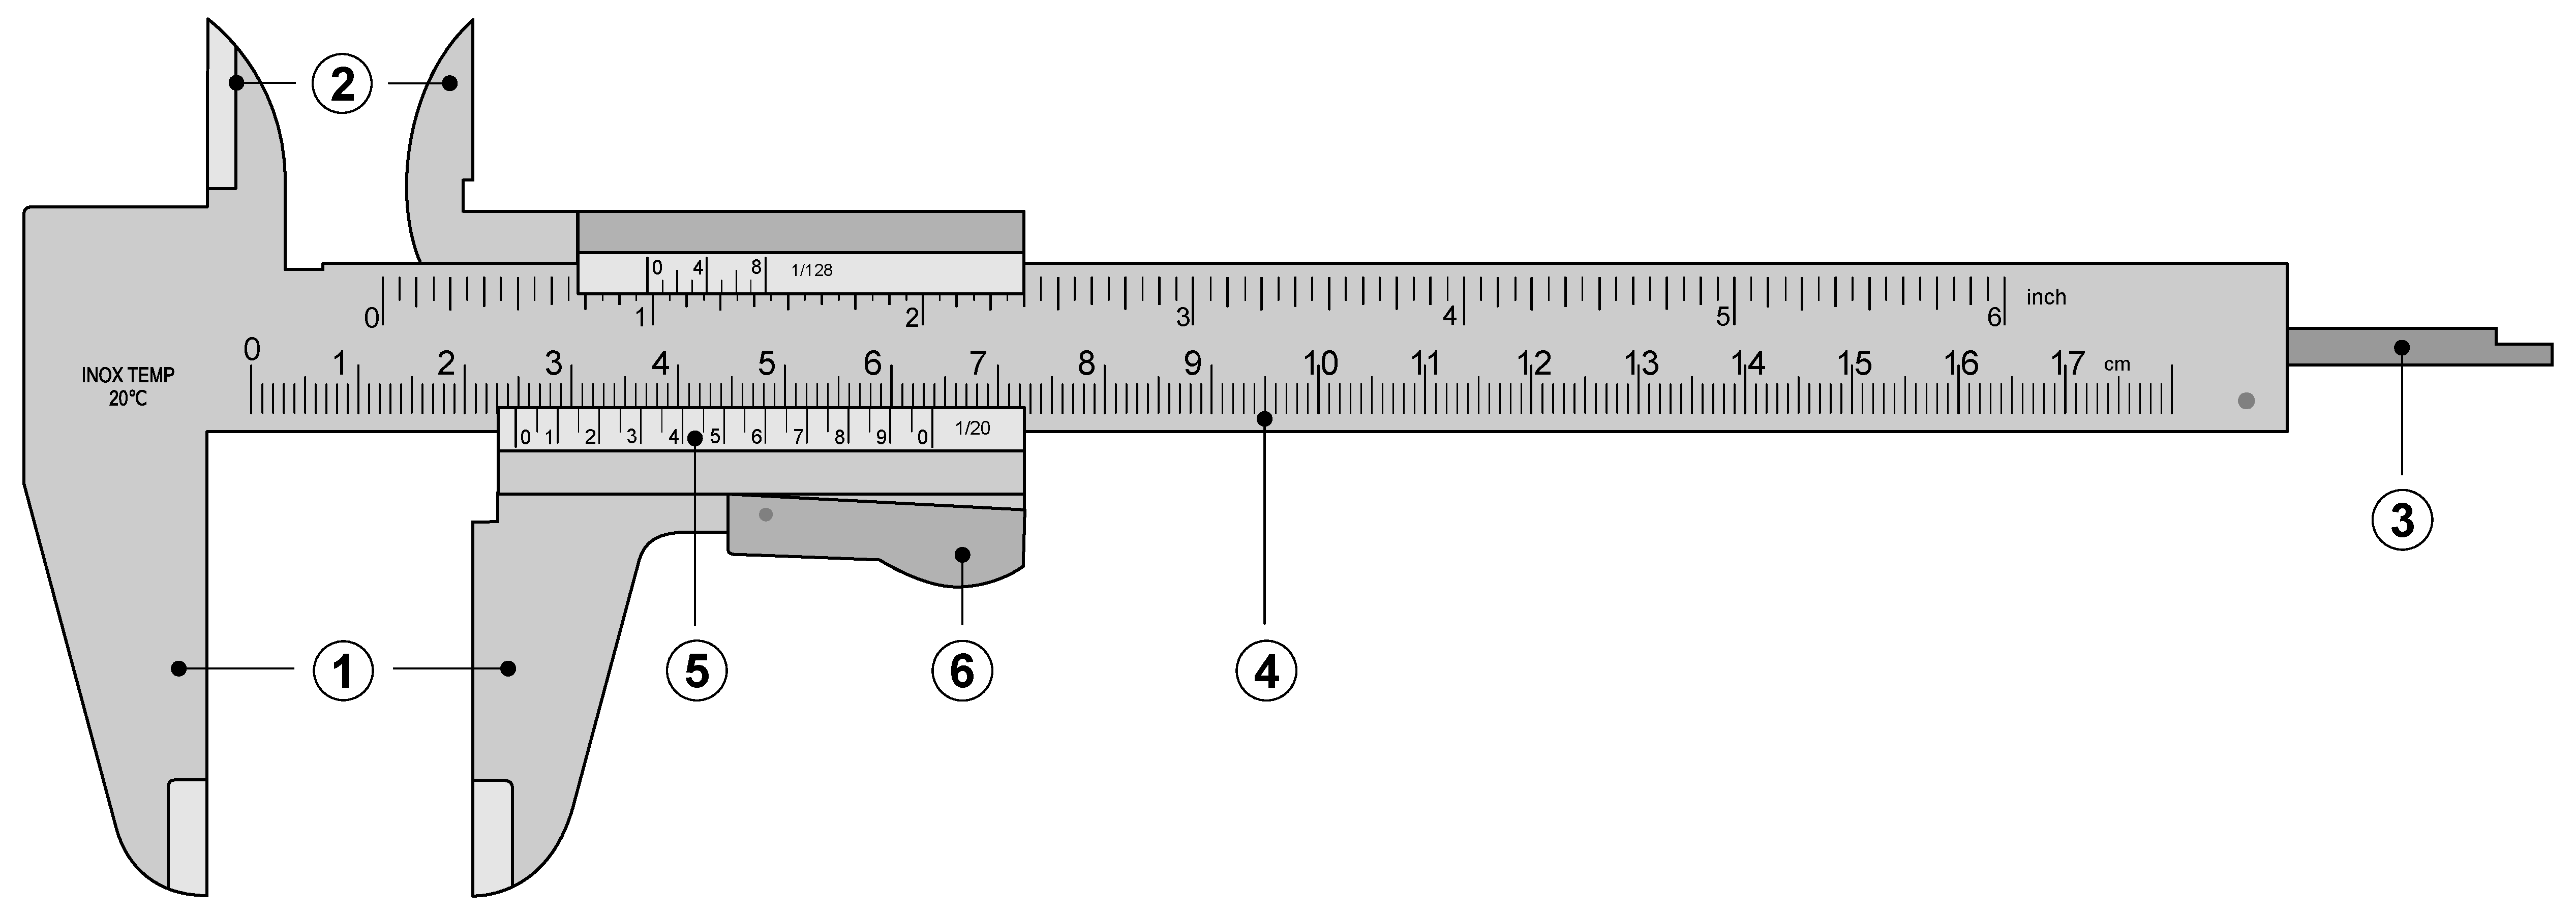
\includegraphics[width=0.75\textwidth]{includes/pictures/vernier.pdf}
  \caption{Calibro universale a nonio.}
  \label{fig::calibro}
\end{figure}

\begin{multicols}{2}
\begin{enumerate}
  \item \textbf{becchi esterni}: per larghezze o diametri esterni;
  \item \textbf{becchi interni}: per larghezze o diametri interni;
  \item \textbf{asta}: per misure di profondità;
  \item \textbf{scala principale}: per misure millimetriche;
  \item \textbf{nonio}: per misurare le frazioni di millimetro;
  \item \textbf{freno}: per il bloccaggio.
\end{enumerate}
\end{multicols}

Per la lettura del calibro, avendo ben posizionato l'oggetto tra i becchi esterni,
si guarda quale tacca della scala principale è \emph{immediatamente precedente} alla
tacca che denota lo \(0\) sul nonio. Il valore di tale tacca è la misura precisa al
millimetro. In seguito si determina quale tacca del nonio corrisponde con la maggior
precisione ad una tacca della scala principale; tale valore sul nonio corrisponderà
alla frazione di millimetro da aggiungere alla misura precedente.\\[1em]
Le formule per il volume che andremo ad utilizzare saranno le seguenti:

\begin{itemize}
  \item \makebox[0.6\linewidth]{cubo di spigolo \(\ell\):\hfill} \(V = \ell^3\)
  \item \makebox[0.6\linewidth]{parallelepipedo rettangolo di spigoli \(a\), \(b\) e \(c\):\hfill} \(V = abc\)
  \item \makebox[0.6\linewidth]{sfera di raggio \(r\) o diametro \(d = 2r\):\hfill} \(V = \dfrac{4}{3} \pi r^3 = \dfrac{1}{6} \pi d^3\)
\end{itemize}


\section{Misure}

Tutte le misure sono state svolte utilizzando un calibro universale a nonio ventesimale,
la cui sensibilità è \(\sigma = \SI{0.005}{\centi\metre}\). I campioni utilizzati sono
stati due cubi, \textbf{C1} e \textbf{C2}, un parallelepipedo \textbf{P} ed una
sfera \textbf{S}. Tutti i valori ottenuti sono riportati in tabella.

\begin{center}\begin{tabular}{ccccccc}
  \toprule
  \textbf{solido} & \textbf{grandezza} & \multicolumn{5}{c}{\textbf{misura} (\si{\centi\metre})} \\
  \midrule
  \textbf{C1} & \(\ell_1\) & \num{1.245} & \num{1.255} & \num{1.250} & \num{1.255} & \num{1.250} \\
  \midrule
  \textbf{C2} & \(\ell_2\) & \num{3.725} & \num{3.700} & \num{3.720} & \num{3.715} & \num{3.720} \\
  \midrule
  \multirow{3}{*}{\textbf{P}} & \(a\) & \num{0.515} & \num{0.510} & \num{0.510} & \num{0.515} & \num{0.510} \\
                              & \(b\) & \num{4.325} & \num{4.320} & \num{4.330} & \num{4.335} & \num{4.320} \\
                              & \(c\) & \num{9.750} & \num{9.750} & \num{9.750} & \num{9.750} & \num{9.750} \\
  \midrule
  \textbf{S} & \(d\) & \num{2.110} & \num{2.105} & \num{2.095} & \num{2.100} & \num{2.110} \\
  \bottomrule
\end{tabular}\end{center}

\section{Analisi dei dati}

Calcoliamo i valori medi (\(\overline{x}\)) e gli errori assoluti (\(\epsilon_x\))
di tutte le misure, quantificando l'errore assoluto tramite la semidispersione
(\(s_x\)), quando questa sia maggiore o uguale alla sensibilità dello strumento,
oppure la sensibilità stessa. Dal momento che ci serviranno per la propagazione
dell'errore, andremo a calcolare anche gli errori relativi (\(e_x\)),
che ricordiamo essere legati agli errori assoluti dalla formula
\(e_x = {\epsilon_x} \, / \, {\overline{x}}\).

\begin{center}\begin{tabular}{cccccc}
  \toprule
  \textbf{solido} & \(x\) & \(\overline{x}\) (\si{\centi\metre}) & \(s_x\) (\si{\centi\metre}) & \(\epsilon_x\) (\si{\centi\metre}) & \(e_x\)\\
  \midrule
  \textbf{C1} & \(\ell_1\) & \num{1.251} & \num{0.005} & \num{0.005} & \num{0.004}\\
  \midrule
  \textbf{C2} & \(\ell_2\) & \num{3.716} & \num{0.012} & \num{0.012} & \num{0.003} \\
  \midrule
  \multirow{3}{*}{\textbf{P}} & \(a\) & \num{0.512} & \num{0.002} & \num{0.005} & \num{0.010}\\
                              & \(b\) & \num{4.326} & \num{0.008} & \num{0.008} & \num{0.0018} \\
                              & \(c\) & \num{9.750} & \num{0.000} & \num{0.005} & \num{0.0005} \\
  \midrule
  \textbf{S} & \(d\) & \num{2.104} & \num{0.008} & \num{0.008} & \num{0.004} \\
  \bottomrule
\end{tabular}\end{center}

Di seguito andiamo a calcolare i volumi e propagare l'errore su di essi.\\[1em]
%
Per il primo cubo:
\begin{align*}
  e_{V_1} &= 3 \, e_{\ell_1} = \num{0.012} \\
  \overline{V_1} &= \left( \overline{\ell_1} \right)^3 = \left( \SI{1.251}{\centi\metre} \right)^3 = \SI{1.958}{\cubic\centi\metre} \\
  \epsilon_{V_1} &= \overline{V_1} \cdot e_{V_1} = \left(\SI{1.958}{\cubic\centi\metre}\right) \cdot \num{0.012} = \SI{0.02}{\cubic\centi\metre} \\
  V_1 &= \SI{1.96(2)}{\cubic\centi\metre}
\end{align*}
%
Per il secondo cubo:
\begin{align*}
  e_{V_2} &= 3 \, e_{\ell_2} = \num{0.009} \\
  \overline{V_2} &= \left( \overline{\ell_2} \right)^3 = \left( \SI{3.716}{\centi\metre} \right)^3 = \SI{51.313}{\cubic\centi\metre} \\
  \epsilon_{V_2} &= \overline{V_2} \cdot e_{V_2} = \left(\SI{51.313}{\cubic\centi\metre}\right) \cdot \num{0.009} = \SI{0.5}{\cubic\centi\metre} \\
  V_2 &= \SI{51.3(5)}{\cubic\centi\metre}
\end{align*}
%
Per il parallelepipedo:
\begin{align*}
  e_{V_\textbf{P}} &= e_{a} + e_{b} + e_{c} = \num{0.012} \\
  \overline{V_\textbf{P}} &= \overline{a} \cdot \overline{b} \cdot \overline{c} = \SI{0.512}{\centi\metre} \cdot \SI{4.326}{\centi\metre} \cdot \SI{9.750}{\centi\metre} = \SI{21.595}{\cubic\centi\metre} \\
  \epsilon_{V_\textbf{P}} &= \overline{V_\textbf{P}} \cdot e_{V_\textbf{P}} = \left(\SI{21.595}{\cubic\centi\metre}\right) \cdot \num{0.012} = \SI{0.3}{\cubic\centi\metre} \\
  V_\textbf{P} &= \SI{21.6(3)}{\cubic\centi\metre}
\end{align*}
%
Per la sfera:
\begin{align*}
  e_{V_\textbf{S}} &= 3 \, e_{d} = \num{0.012} \\
  \overline{V_\textbf{S}} &= \frac{1}{6} \pi \left(\overline{d}\right)^3 = \frac{\pi}{6} \left( \SI{2.104}{\centi\metre} \right)^3 = \SI{4.877}{\cubic\centi\metre} \\
  \epsilon_{V_\textbf{S}} &= \overline{V_\textbf{S}} \cdot e_{V_\textbf{S}} = \left(\SI{4.877}{\cubic\centi\metre}\right) \cdot \num{0.012} = \SI{0.06}{\cubic\centi\metre} \\
  V_\textbf{S} &= \SI{4.88(6)}{\cubic\centi\metre}
\end{align*}

\section{Conclusioni}

Attraverso questa esperienza abbiamo messo in pratica le nostre conoscenze di
propagazione dell'errore e siamo entrati in contatto con uno strumento di misura
a noi nuovo, il calibro.

\end{document}
